\chapter{IoT}
Internet delle cose (Internet of Things, IoT) è un paradigma riferito
all’estensione di internet al mondo degli oggetti. Nel 1999 il ricercatore
britannico Kevin Ashton durante una presentazione teorizzò  per primo un mondo
nel quale oggetti dotati di sensori, interagiscono utilizzando la rete.  La
continua evoluzione delle tecnologie wireless e satellitari ha permesso
l'ideazione di oggetti sempre più connessi, in grado di generare una grande mole
di informazioni e dati. Oltre ai computer smartphone e tablet, sempre più
oggetti di uso quotidiano dispongono di una connessione ad internet. Smartwatch
e smart band , lampadine e prese elettriche "intelligenti" ,  sono già da tempo
reperibili nel mercato con un prezzo accessibile a tutti .  Data la bassa
complessità del hardware implementato in questi devices, essi necessitano di
appoggiarsi ad un server esterno per l'elaborazione dei dati.  Sfruttando la
connessione ad internet, gli oggetti riescono ad instaurare uno scambio di dati
bidirezionale tra loro ed il server; infatti l'oggetto dopo aver trasformato gli
input ricevuti dal mondo esterno in dati, invia l'informazione al server il
quale, dopo un'elaborazione degli stessi, formula dei comandi da inviare
all'oggetto.
\\
\begin{figure}[h]
        \centering 
                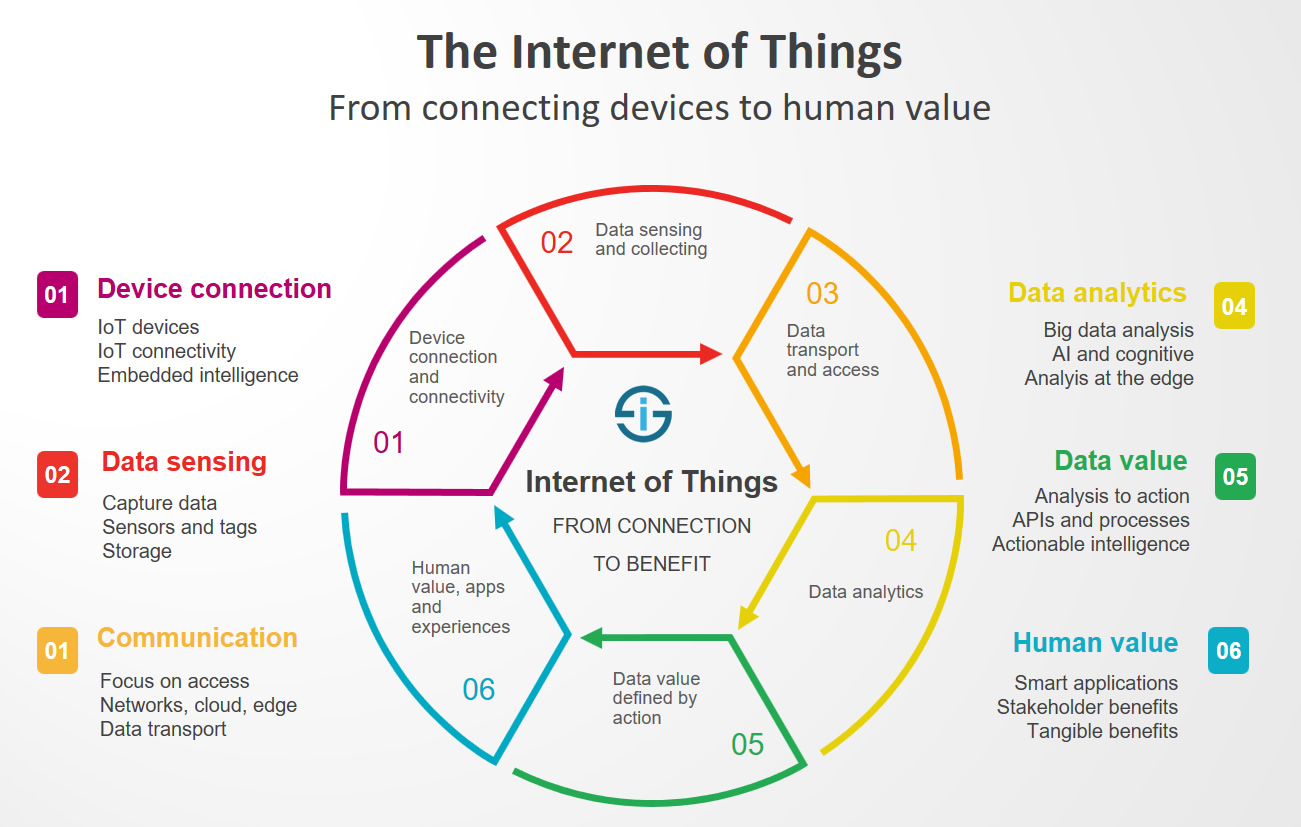
\includegraphics[width=10cm]{Orignal/IoT-c1.jpg}
        \caption{Numero di dispositivi per anno}
\end{figure}
Nel mondo dell’IoT i dati condivisi sono in
continuo aumento, innescando una serie di progressi importanti anche da un punto
di vista economico, andando ad incidere  significativamente sulla “catena del
valore” (value chain). Attraverso lo studio delle informazioni presenti ,si
potrà  aumentare l’efficienza di un servizio oppure  migliorare la user experience di una applicazione ecc.  
Muovendoci
verso un modo sempre più connesso, nove problematiche riguardanti la privacy e
la sicurezza emergo.  Molto spesso per ridurre i costi di produzione e di
sviluppo di questi oggetti smart, le aziende tendo a ridurre gli investimenti
nell'R\&D (Ricerca e Sviluppo), andando a produrre dispositivi con un software no
aggiornato o con componenti hardware di bassa qualità.
Sono già numerosi i casi di attacchi hacker i quali, avvalendosi delle falle
presenti nei dispositivi, riescono ad entrare in possesso della rete ai cui il
dispositivo è collegato .

\section{La diffusione dell'Internet delle cose}
Nel 2008 il numero di oggetti quali personal-computer, server, telefoni cellulari,
connessi ad internet ha superato il numero di persone presenti nell'intero
pianeta. Il continuo sviluppo tecnologico, la sempre maggior facilità d'uso e
l'abbattimento dei costi, ha reso disponibile al mondo consumer tecnologie che
fino a poco tempo fa erano destinate ad aziende ed università. 
Con l'avvento dell'IoT si prevede una crescita esponenziale di devices connessi
ad Internet;  secondo  una stima da parte di Gartner, il numero di smart
device presenti nell'anno 2020, sarà superiore a 20 miliardi \cite{gartner2016}
Inoltre è proprio il lato consumer che ne fa da padrone con ben \$5.2 miliardi
di dollari investi in prodotti quali smart TV, set-top box e smart cars.
\\
\begin{table}[h]
        \centering
        \begin{tabular}{l|c|c|c|c}
                \textbf{Categoria}  & 2016 & 2017 & 2018 & 2019 \\
                \hline
                \emph{Consumer}  & 3963 & 5244,3 & 7063,3 & 12863 \\
                \emph{Business}  & 1418 & 2135.4 & 4152,7 & 6171  \\
                \emph{Totale }   & 6381 & 8380   & 11196  & 20415 \\
        \end{tabular}
        \caption{Stima di dispositivi IoT (Milioni di unità)
        Gartner\cite{gartner2016}}
\end{table}
\\
\begin{figure}[h]
        \centering 
                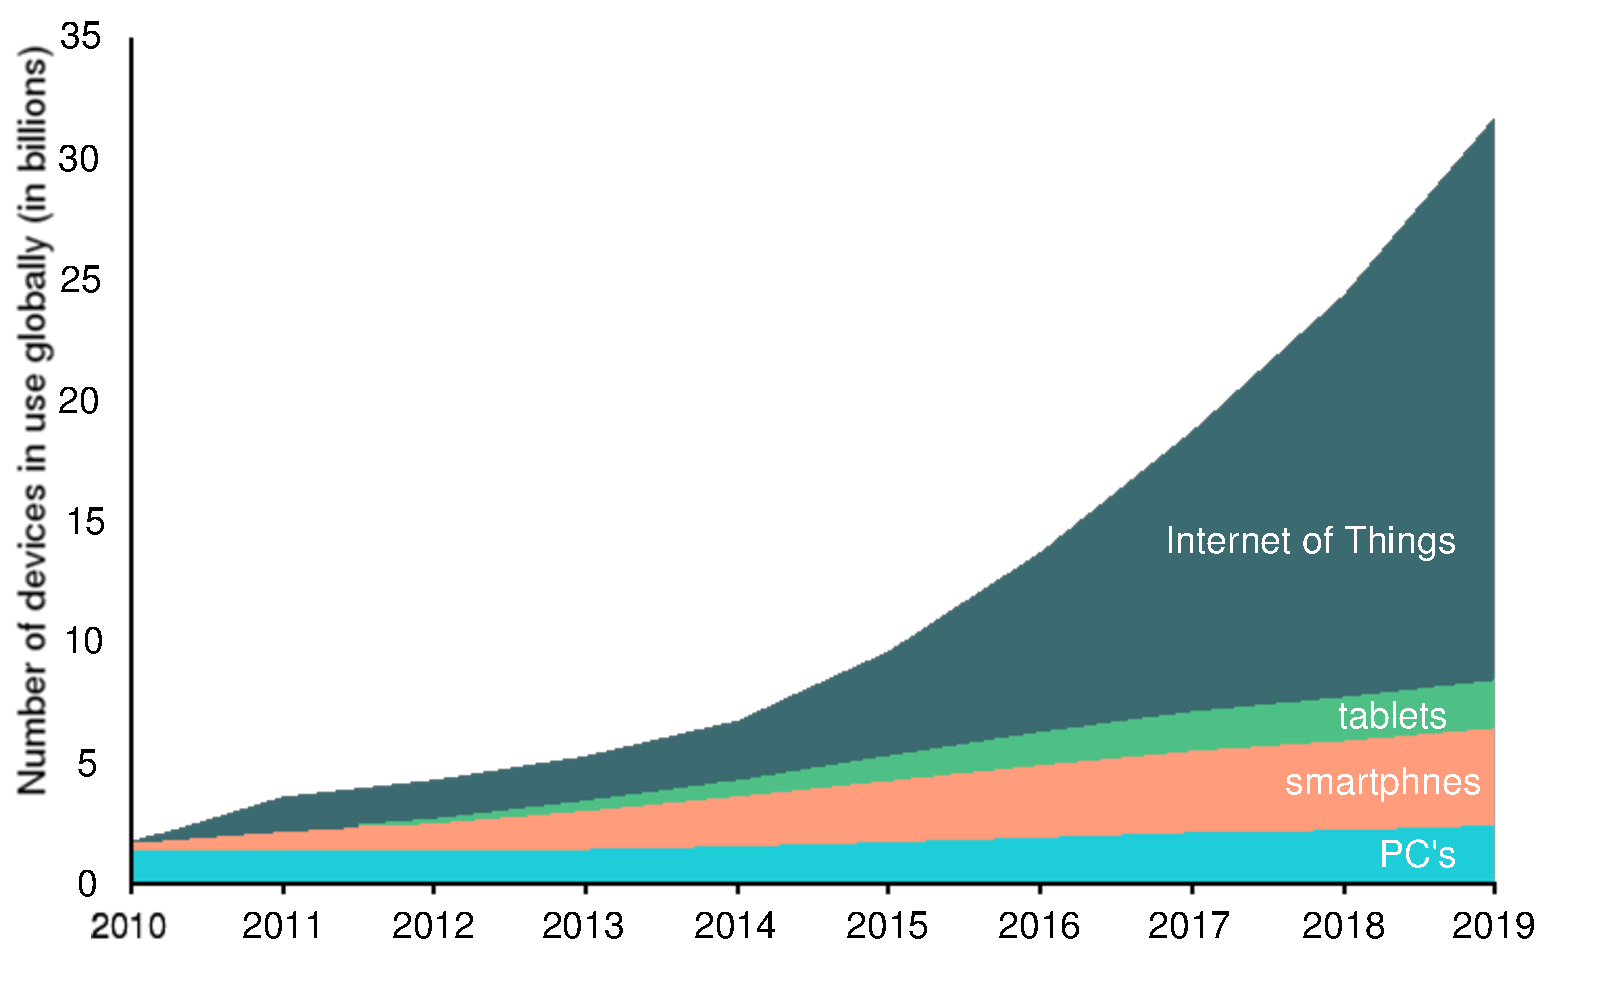
\includegraphics[width=10cm]{iot_devices}
        \caption{Numero di dispositivi per anno}
\end{figure}
\section{Business}
Considerando le statistiche precedenti immediato notare come l'IoT sia un
business che agisce in maniera tutti i settori in maniera trasversale.
Se da molto tempo si parla di domotica e smart city, tramite l'abbattimento dei
costi dei vari dispositivi nuovi mercati e nuove possibilità di investimento
sono nate. Prendiamo come esempio l'agricoltura di precisione, che grazie a
sensori in grado di estrapolare dati come l'umidità del suolo, l'indice di
piovosità e l'umidità delle foglie, 
permettono all'agricoltore, tramite l'analisi dei dati raccolti, di capire
quando è il momento di intervenire per il trattamento delle colture; permettendo
l'incanalazione delle risorse impiegate, aumentando la produttività . 
Questo voleva essere solo un esempio della vastità delle opportunità  offerte
dall'IoT. Gartner, si stima che entro il 2020 la cifra
investita nell'idustria del IoT sarà pari a circa \$3,000,000 milioni di dollari
con un investimento annuo di circa \$500,000 milioni di dollari
\cite{gartner2016}. 

\section{Big Data}
Oltre all'innumerevole quantità di dati che verrà prodotta da questi milioni di
devices intelligenti, noi stessi,  navigando il web produciamo una grande
quantità di dati. Con il  termine Big Data si vuole rappresentare l'insieme di
tutti i dati eterogenei che ogni giorno vengono prodotti e scambiati nella rete.
Con il progredire della tecnologia il dataset (aggregazione di dati) a
disposizione delle aziende è in continuo aumento.
Secondo un articolo pubblicato da Verizon, si stima che il 92\% delle aziende
usa meno del 25\% dei dati raccolti e che solo la metà  di esse prevede di
riuscire a fare fruttare più del 25\% di dati nei prossimi due anni
\cite{Verizon}.  Con “Data mining” o "Data analytics"  si identificano tutte le
tecniche e le metodologie finalizzate all’estrazione di sapere e conoscenza
partendo da una vasta mole di dati.
L’enorme disponibilit`a di ogni sorta di informazione `e una prospettiva al-
apre innumerevoli scenari di ricerca; ad esempio, predire con largo anticipo la
diffusione di una malattia epidemica permette di prioritizzare gli interventi
sanitari preventivi nelle aree pi`u bisognose.  Pur avendo benefici
incontestabili, per`o, si presenta la possibilit`a, seppur remota, di risalire
alle fonti di questa conoscenza e ai dati  personali di singoli, specifici
individui.  Con “dato personale” si intende qualsiasi informazione che
identifica o rende identificabile una persona fisica.  Generalmente si distingue
tra dati  identi- ficativi (dati anagrafici, fotografie, ...)  e dati sensibili
, che possono rivelare “l’origine  razziale  ed  etnica,  le  convinzioni
religiose,  filosofiche  o  di  altro Oggigiorno, gran parte delle aziende sono
impegnate nell'attuazione del data mining, considerandolo un investimento a
lungo termine. 
E molto comune che un dataset includa, nella sua forma originale, infor-
mazioni che sono riconducibili a specifici individui - un nome, una data di
nascita, un indirizzo IP. Ci`o diventa potenzialmente pericoloso nel momento
in  cui  si  dispone  di  una  chiave  per  collegare  dati  su  uno  stesso  individuo
provenienti  da  fonti  diverse  -  informazioni  sanitarie,  preferenze  e  opinioni
espresse sui social network, dati collegati alle spese online e ai metodi di pa-
gamento.


\section{La tecnologia alla base dell'IoT} 
Nell'industria il concetto di M2M (Machine to Machine) non è un concetto nuovo,
già Kevin Ashton, durante la presentazione in cui introdusse il termine IoT,
comprese le potenzialità della tecnologia RFID applicate alla supply chain. Dal
1999 ad oggi molte cose sono cambiate, ma molte domande non hanno ancora trovato
una risposta. Come accadde agli albori di Internet, quello che manca al modo
dell'IoT è una standardizzazione dei protocolli e del linguaggio con cui questi
oggetti devono comunicare. Una possibile archittettura 
l'IoT necessita anche di uno
una architettura bottom up suddivisa in tre livelli.
\begin{figure}[h]
        \centering 
                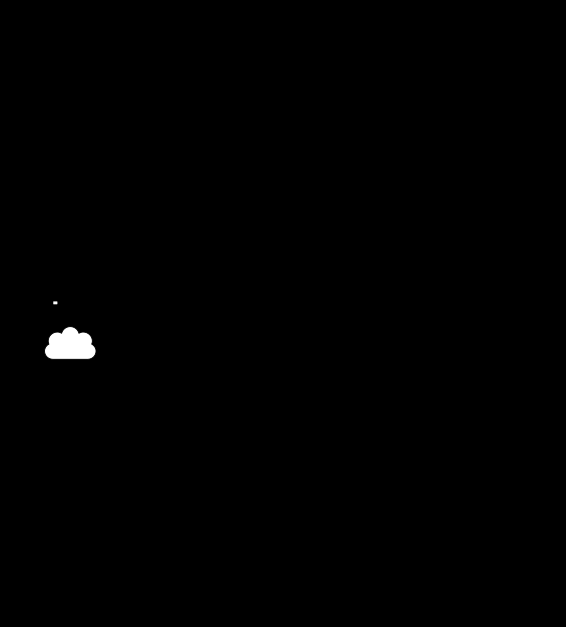
\includegraphics[width=10cm]{three-layer}
        \caption{Layer del IoT}
\end{figure}
\begin{itemize}
\item \textbf{Device layer} o sensor layer, è il layer più basso. Esso raggruppa
tutti i gli oggetti "smart". Questo layer è quello che mette in comunicazione il
mondo reale con gli atri layer superiori. A loro spetta lo scopo di convertire
una misura fisica in un segnale interpretabile da altri calcolatori.
La maggior parte di questi sensori, utilizzerà una connessione Bluetooth,
ZigBee, Wifi o una si baserà su una rete LPWAN per comunicare il dato al layer
superiore.
\item \textbf{Network layer} o mediation layer raggruppa l'intera infrastruttura
di rete e gateway che ricevono i dati da i vari sensori. Questo layer è
semplicemente un layer di mediazione dove l'informazione (dato) non viene altera
ma semplicemente trasmesso all'Application layer.
\item \textbf{Application layer} è il layer nel quale l'informazione viene
immagazzinata ed elaborata. Questo layer è il più importante, e qui dove il dato
viene trasformato da una semplice misurazione fisica ad una possibile revenue
per l'azienda che lo gestisce.\improvement{Riscrivere}
\end{itemize}


Già alcune aziende del calibro di Samsung con la
piattaforma \href{https://www.artik.io}{artik}  , Zigbee con
\href{https://www.speakdotdot.com/dotdot/}{DotDot} e Google con
\href{https://developers.nest.com/weave/}{Weave}, stanno cercando di imporsi per
creare un .
Ognuna di queste soluzioni punta a creare un linguaggio comune per i vari
oggetti smart, in questo modo il sviluppo e l'integrazione risulterà più
semplice, velocizzando il time to market dei prodotti.
Oltre alla mancanza di un linguaggio comune , Con questa tesi si vuole approfondire lo stato dell'arte del network layer
andando a esporre le principali tecnologie ad oggi presenti sul mercato. In
particolare verrà posta l'attenzione sulla tecnologia LoRaWAN e l'integrazione
con il framework Kura/ESF sviluppato da Eurotech.



